\documentclass[12pt]{article}

\usepackage{graphicx}

\title{Observations of Kepler Binary Stars}
\date{2016 June 1}
\author{Brendon Walter}

\begin{document}
	\maketitle
	
	\section{Abstract}
	
	The Kepler mission is set to find planets orbiting stars outside our solar system. In 2011, the Kepler mission released a catalog of all the eclipsing binaries that they had found so far. Using this catalog, I sorted the binaries by the depth of its primary eclipse with the idea that a deeper eclipse would result in more notable difference in magnitude. I then wrote a script in Python which would calculate the time and date of the next eclipse for each system. As so many of the systems had periods of less than 1 day, there would often be several eclipses happening in one hour. Observations were made with an Optec SSP-3 photometer on a 16 inch telescope at the Stickney Observatory on the Bennington College Campus. For the first two nights of data collecting, I only observed the counts given from the star. On the third night, I recorded a count of the night sky with no objects in it. No good results were obtained due to several reasons.
	
	\section{Kepler Eclipsing Binaries Catalog}
	
	The Kepler mission is set to find planets orbiting stars outside our solar system. The area of the sky that it's studying contains over 156,000 stars being observed to find any dips in apparent magnitude which would suggest that there is a planet orbiting the star. As is expected, not all of the stars that feature a dip are due to exoplanets.\footnote{Prsa et al (2011)} Many of these stars are eclipsing binary systems - solar systems which are made up of two stars which eclipse one another when viewed from Earth.
	\\\\
	In 2011, the Kepler mission released a catalog of all the eclipsing binaries they had found so far. The catalog, currently on its 3rd version, contains information about the binary's coordinates, the width and depth of the primary and secondary minima, temperatures of the stars, and more.\footnote{The full catalog is online at http://keplerebs.villanova.edu/}
	
	\section{Calculating Eclipse Times}
	
	Using the Kepler Eclipsing Binaries catalog, I sorted the binaries by the depth of its primary eclipse with the idea that a deeper eclipse would result in more notable difference in magnitude. From the sorted list, I then selected the top fifty systems which had a period of less than four days. This length of time was chosen because I planned on observing at least three eclipses for several systems within a month time frame. 
	\\\\
	I then wrote a script in Python which would calculate the time and date of the next eclipse for each system. These times were calculated from the Julian date at which the maximum depth of the primary minima was observed as well as the width of the minima, given in the catalog in terms of days. The time of the peak of the next eclipse was then converted from Julian date to the Gregorian Date in Eastern Daylight Time. The program then wrote a list of the 50 stars sorted by time of the next eclipse to a text file. In addition to the next eclipse, output included the Kepler ID number, the period of the system in days, the apparent magnitude of the system, and its coordinates. A sample of the output can be seen in Figure 1.
	\begin{figure}
		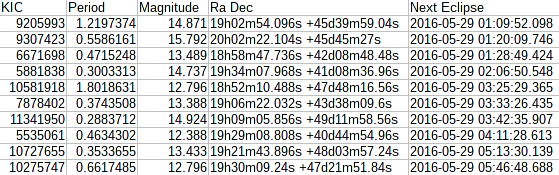
\includegraphics[width=\textwidth]{./images/nextEclipses.png}
		\caption{Sample output of the program which would calculate the times of the next eclipses.}
	\end{figure}
	
	\section{Data Collection}
	
	As so many of the systems had periods of less than 1 day, there would often be several eclipses happening in one hour. This made it easy to catch any of the eclipses as I would wait at most thirty minutes before an eclipse would begin. 
	\\\\
	Observations were made with an Optec SSP-3 photometer on a 16 inch telescope at the Stickney Observatory on the Bennington College Campus. Integration time was set to 10 seconds and the gain set to either 10 or 100. I aimed to record the total count around every 5 minutes.
	\\\\
	For the first two nights of data collecting, I only observed the counts given from the star. On the third night, I recorded a count of the night sky with no objects in it.
	
	\section{Results \& Discussion}
	
		\begin{figure}
			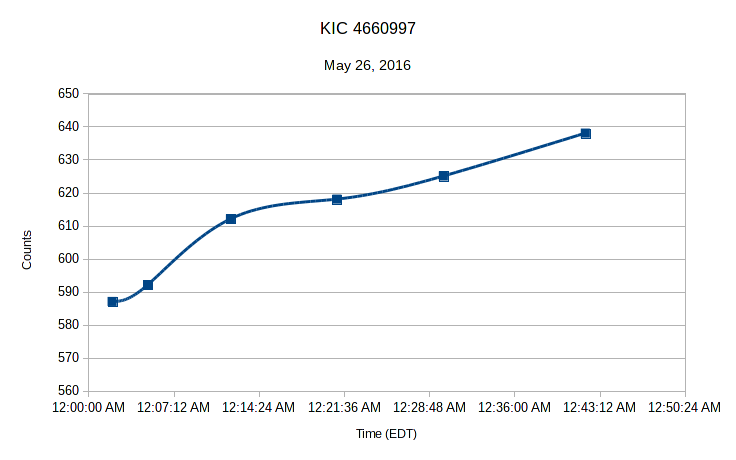
\includegraphics[width=\textwidth]{./images/KIC4660997.png}
			\caption{Observations made on May 26 starting at 12:02 am EDT. The maximum depth of the eclipse was scheduled to happen at 12:23 am EDT and has a magnitude of 12.37. The gain on the photometer was set to 10 and integration time to 10 seconds. The moon started to rise at 12:00am, right when I started observations.}
		\end{figure}
		
		\begin{figure}
			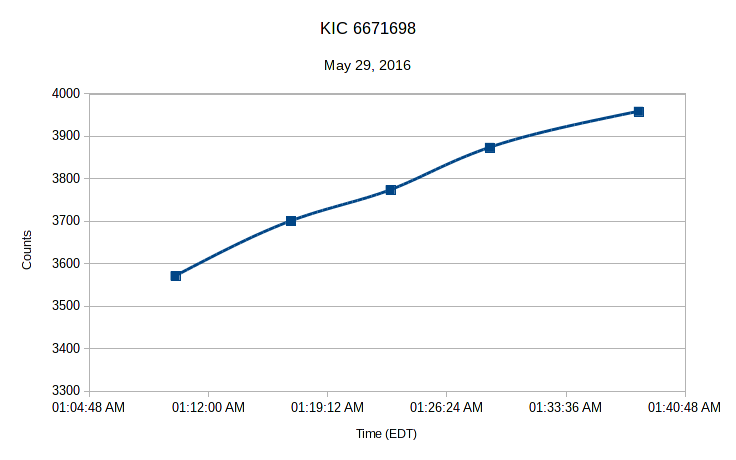
\includegraphics[width=\textwidth]{./images/KIC6671698.png}
			\caption{Observations made on May 29 starting at 1:10 am EDT. The maximum depth of the eclipse was scheduled to happen at 1:28 am EDT and has a magnitude of 13.5. The gain on the photometer was set to 100 and the integration time to 10 seconds. The moon started to rise at 1:22am, once again right around when I started to observe.}
		\end{figure}
		
		\begin{figure}
			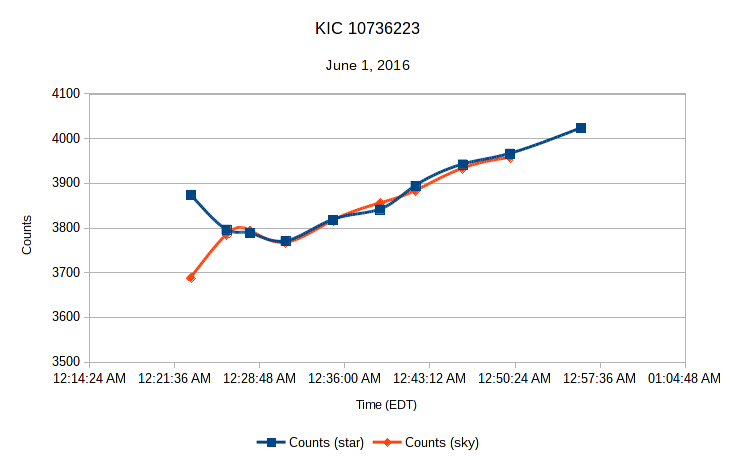
\includegraphics[width=\textwidth]{./images/KIC10736223.png}
			\caption{Observations made on June 1 starting at 12:23 am EDT. The maximum depth of the eclipse was scheduled to happen at 12:28 am EDT and has a magnitude of 13.7. The gain on the photometere was set to 100 and the integration time to 10 seconds. The moon was scheduled to rise at 3:05 am - this leads to the question as to why the counts even for the sky continued to steadily rise.}
		\end{figure}
	
	No good results were obtained. This was caused by several reasons:
	\begin{enumerate}
		\item There were few days in May with clear skies. Of the days with clear skies, I was only able to observe during some of them.
		\item Many of the stars I chose had magntiudes of over 14, and often times the stars were not the brightest stars in the field. This made it difficult to know which star I was looking at and even when I did have a good idea of which star it was, I often could only see the star with my peripheral vision because it was so faint. For the observations made on June 1, 2016, I could not see the star at all and had to trust that the telescope was pointing at the correct object.
		\item On the three nights that I was able to find what I believe to be the star and was able to center it and gather data, the moon rose during observations and caused the sky to become brighter. The result of this was that instead of observing a decrease in total counts in the photometer as expected, what happened instead was that the counts continued to rise throughout the primary minima.
	\end{enumerate}
	There were several things that could have been done differently in order to obtain better results:
	\begin{enumerate}
		\item There isn't much that can be done about cloudy days, other than not living in New England.
		\item When choosing the stars to use, an additional parameter could have been the magnitude of the star. Additionally, the program I wrote to calculate the eclipse could be easily modified to automatically choose stars from the entire list making it easier to specify multiple criteria such as Period $<$ 4 and Magnitude $>$ 13.
		\item On the third attempt at observing, I gathered a reading of the night sky with no stars in the field of view. This made it so that I could calibrate the star against the dark sky making it so that outside influences, such as the moon, didn't have as much of an impact. This process should have been applied to the other nights of observations.
	\end{enumerate}
	Figures 2-4 plot the number of counts I obtained during each night of observations and at what times. Figure 4 is the only plot out of the three which displays a dip in overall brightness around where the maximum depth was expected to happen.
	
	\section{Citations}
	
	 Prsa, Andrej, Natalie Batalha, Robert W. Slawson, Laurance R. Doyle, William F. Welsh, Jerome A. Orosz, Sara Seager, Michael Rucker, Kimberly Mjaseth, Scott G. Engle, Kyle Conroy, Jon Jenkins, Douglas Caldwell, David Koch, and William Borucki. \textit{Kepler Eclipsing Binary Stars. I. Catalog And Principal Characterization Of 1879 Eclipsing Binaries In The First Data Release.} The Astronomical Journal 141.3 (2011): 83. Web. 
	
\end{document}